\documentclass[a4paper]{article}

% Packages
\usepackage[14pt]{extsizes}
\usepackage[T2A]{fontenc}
\usepackage[russian]{babel}
\usepackage[left=20mm, top=15mm, right=15mm, bottom=20mm]{geometry}
\usepackage{graphicx} % For images
\usepackage{amsmath, amssymb} % For equations
\usepackage{booktabs} % For better tables
\usepackage{pgfplots} % For plotting graphs
\usepackage{xcolor} % For color support
\usepackage{caption} % For captioning tables and figures
\usepackage{float} % For precise float placement (images, tables)
\usepackage{array} % For better table management
\usepackage{booktabs}
\usepackage{hyperref}
\usepackage{longtable}
\pgfplotsset{compat=1.17}

% Importing custom definitions (lstset, tikzset, etc.)
% % listing for programming code blocks
% listing for Python code blocks
\lstset{
	language=python,                 % Programming language
	basicstyle=\ttfamily\small,      % Adjust font size
	keywordstyle=\color{blue}\bfseries,  % Style for keywords
	stringstyle=\color{red},         % Style for strings
	commentstyle=\color{gray}\itshape, % Style for comments
	morecomment=[l][\color{magenta}]{\#}, % Special comment style for Python comments
	breaklines=true,                 % Line breaking in long lines
	numbers=left,                    % Line numbering on the left
	numberstyle=\tiny\color{gray},   % Style for line numbers
	frame=single,                    % Code frame
	showstringspaces=false,          % Don't show spaces in strings
	captionpos=b,                    % Caption position (b = bottom)
	tabsize=4,                       % Adjust tab spacing
	rulecolor=\color{black},         % Color of the frame
	emph={self},                     % Specific highlighting for keywords like 'self'
	emphstyle=\color{teal},          % Style for emphasized words (like 'self')
}

% \input{../common/tikzset.tex}

% -------------------------------

\begin{document}

% Title page
\input{../common/title-old.tex}
\thispagestyle{empty}

\newpage
\pagestyle{plain}
\setcounter{page}{1}

% -------------------------------

% autogenerated table of contents
\linespread{0.9}
\tableofcontents
\linespread{1}

% -------------------------------

\newpage
\section*{Цель работы}
Изучение методов обработки и статистического анализа результатов измерений на примере
заданной числовой последовательности путем оценки числовых моментов и выявления свойств
последовательности на основе корреляционного анализа, а также аппроксимация закона
распределения заданной последовательности по двум числовым моментам случайной величины.

% -------------------------------

\section{Построение графика значений для заданной числовой последовательности}

График данной последовательности имеет следующий вид:

\begin{figure}[H]
	\centering
	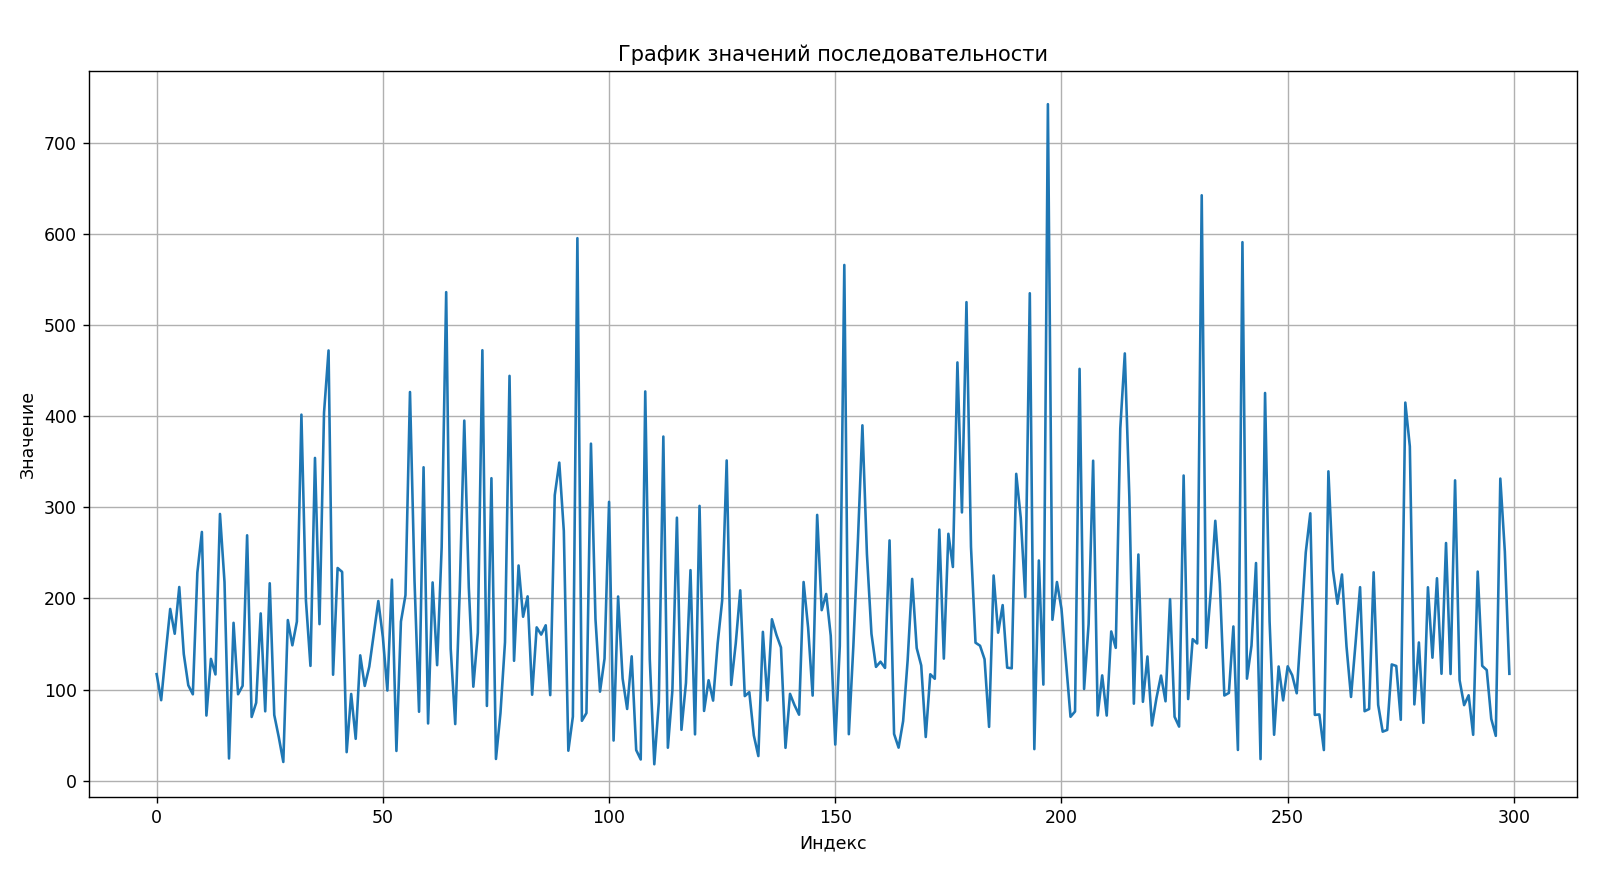
\includegraphics[width=0.9\textwidth]{data/sequence.png}
	\caption{График числовой последовательности}
\end{figure}

Очевидно, что данная последовательность не является возрастающей/невозрастающей, равно как и
не является убывающей/неубывающей. Можно было бы сказать, что последовательность отдалённо похожа на периодическую,
однако у неё отсутствует какой-либо повторяющийся за единицу времени паттерн.

\section{Автокорреляционный анализ}

\begin{table}[H]
	\centering
	\caption{Автокорреляционные коэффициенты (АК) для заданной и сгенерированной ЧП}
	\resizebox{\textwidth}{!}{

		\begin{tabular}{|c|c|c|c|c|c|c|c|c|c|c|}
			\hline
			\textbf{Сдвиг ЧП}                      & \textbf{1} & \textbf{2} & \textbf{3} & \textbf{4} & \textbf{5} & \textbf{6} & \textbf{7} & \textbf{8} & \textbf{9} & \textbf{10} \\
			\hline
			\textbf{К-т АК для заданной ЧП}        & -0.0206    & -0.0099    & 0.0579     & 0.0680     & -0.0160    & -0.0047    & 0.0170     & -0.0307    & -0.0334    & -0.0260     \\
			\hline
			\textbf{К-т АК для сгенерированной ЧП} & -0.0464    & 0.0167     & 0.0242     & -0.0350    & 0.0909     & -0.0560    & -0.0495    & -0.0452    & -0.0632    & -0.0089     \\
			\hline
			\textbf{\%}                            & 125.243    & -268.687   & -58.204    & -151.471   & -668.125   & 1091.49    & -391.176   & 47.231     & 89.222     & -65.769     \\
			\hline
		\end{tabular}

	}
\end{table}


\begin{figure}[H]
	\centering
	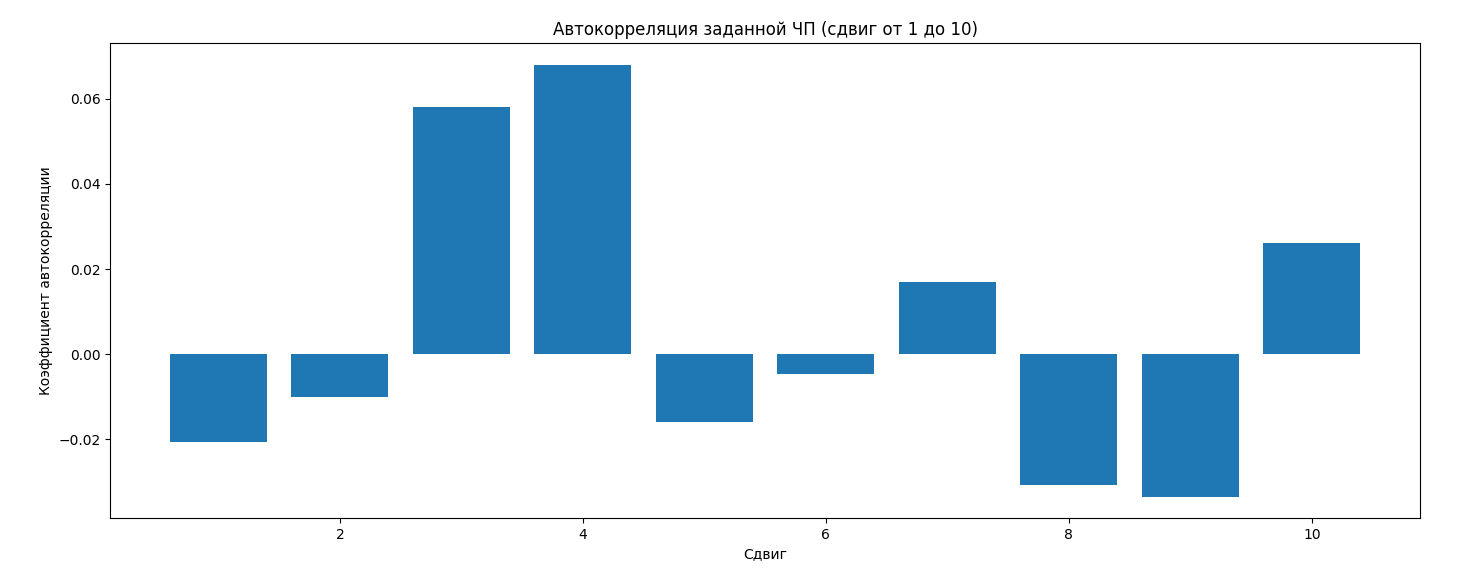
\includegraphics[width=0.8\textwidth]{data/auto_corellation-1.png}
	\caption{Автокорреляционный анализ для заданной последовательности}
\end{figure}

Автокорреляция в сути своей показывает зависимость между текущими данными и предыдущими значениями для выявления
тенденций в последовательностях (т.е. чтобы по предыдущим значениям мы имели возможность предсказать
следующие).

В качестве порогового значения, превышение которого говорит о том, что последовательность неслучайна, нами было выбрано
значение 0.2, и, как мы убедились во время проведения работы, ни для одного из сдвигов коэффициенты автокорреляции не
превышали даже 0.1, из чего мы можем предполагать, что заданная числовая последовательность является случайной.

\begin{figure}[H]
	\centering
	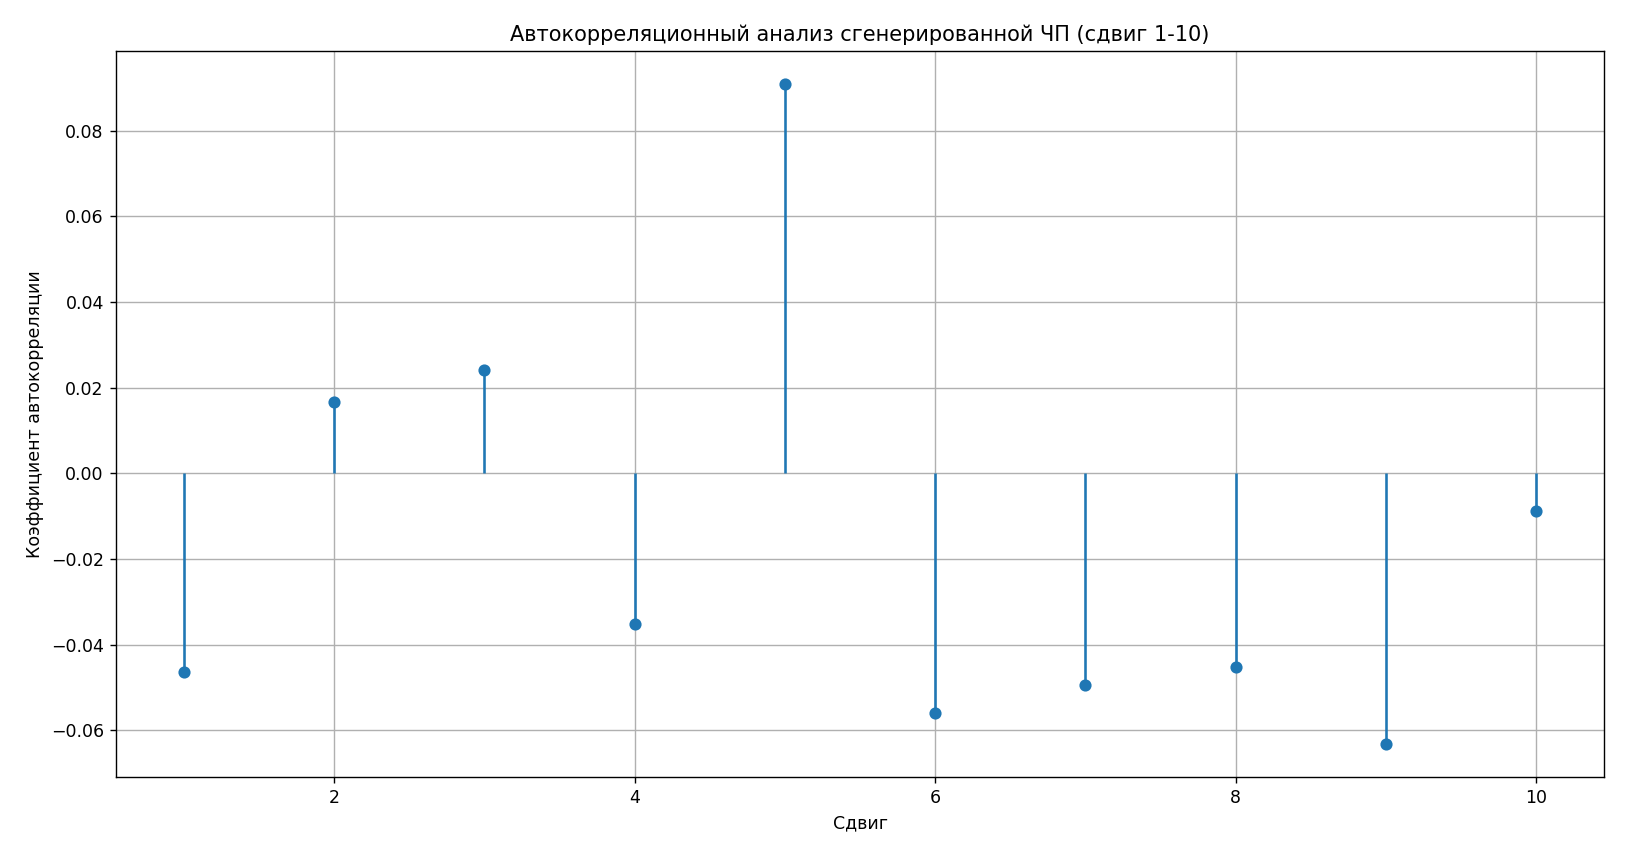
\includegraphics[width=0.75\textwidth]{data/auto_corellation-2.png}
	\caption{Автокорреляционный анализ для сгенерированной последовательности}
\end{figure}

Автокорреляционный анализ сгенерированной числовой последовательности даёт нам аналогичные результаты: ни одно из
значений коэффициентов автокорреляции не превышало 0.1, не говоря уже о 0.2, из чего мы можем делать вывод, что
генерируемая нами последовательность не только случайна, но и приближена к заданной.


\section{[old] Рассчитать числовые моменты заданной ЧП}
\begin{itemize}
	\item Математическое ожидание:
	      \[
		      \mu = \frac{1}{n} \sum_{i=1}^{n} X_i
	      \]
	      где \( X_i \) — элементы последовательности, \( n \) — количество элементов.

	\item Дисперсия:
	      \[
		      \sigma^2 = \frac{1}{n-1} \sum_{i=1}^{n} (X_i - \mu)^2
	      \]
	      где \( \mu \) — математическое ожидание, \( n-1 \) — степень свободы для корректировки выборки.

	\item Среднеквадратическое отклонение:
	      \[
		      \sigma = \sqrt{\sigma^2}
	      \]

	\item Коэффициент вариации:
	      \[
		      CV = \frac{\sigma}{\mu} \times 100
	      \]
	      Коэффициент вариации показывает относительное отклонение данных от среднего значения в процентах.
\end{itemize}


\section{Построение доверительных интервалов}

Пусть для некоторой случайной величины \( X \) в результате имитационного моделирования получена несмещенная оценка математического ожидания \( \tilde{m} \) и оценка дисперсии \( \tilde{D} \), рассчитанные по следующим формулам:

\[
	\tilde{m} = \frac{1}{n} \sum_{i=1}^{n} X_i
\]
\[
	\tilde{D} = \frac{1}{n-1} \sum_{i=1}^{n} (X_i - \tilde{m})^2
\]

где \( X_i \) — значения случайной величины, \( n \) — количество измерений.

Для построения доверительного интервала с доверительной вероятностью \( p \) определим величину погрешности \( \epsilon_p \), которая вычисляется по формуле:

\[
	\epsilon_p = t_p \cdot \sigma_m = t_p \cdot \frac{\sqrt{\tilde{D}}}{\sqrt{n}}
\]

где \( t_p \) — коэффициент, найденный по таблице для выбранного уровня доверия \( p \), \( \sigma_m \) — оценка стандартного отклонения математического ожидания.

\subsection{Доверительный интервал для математического ожидания}

Доверительный интервал для математического ожидания с заданной доверительной вероятностью \( p \) задается как:

\[
	[m_\text{н}, m_\text{в}] = [\tilde{m} - \epsilon_p, \tilde{m} + \epsilon_p]
\]

где:
\begin{itemize}
	\item \( m_\text{н} = \tilde{м} - \epsilon_p \) — нижняя граница доверительного интервала,
	\item \( m_\text{в} = \tilde{м} + \epsilon_p \) — верхняя граница доверительного интервала.
\end{itemize}

Таким образом, с вероятностью \( p \) истинное значение математического ожидания находится в интервале \( [m_\text{н}, m_\text{в}] \).

\subsection{Относительная погрешность}

Относительная погрешность оценки математического ожидания \( \delta \) рассчитывается по следующей формуле:

\[
	\delta = \frac{\epsilon_p}{\tilde{m}} \times 100
\]

где \( \epsilon_p \) — половина длины доверительного интервала. Это значение показывает, насколько сильно точечная оценка отличается от истинного значения в процентах.

\subsection{Пример расчета}

Предположим, что в результате 300 измерений случайной величины \( X \) были получены следующие оценки:
\[
	\tilde{m} = 50, \quad \tilde{D} = 45816
\]
Тогда оценка стандартного отклонения математического ожидания:

\[
	\sigma_m = \frac{\sqrt{\tilde{D}}}{\sqrt{300}} = 28.57
\]

Для доверительной вероятности \( p = 0.95 \), коэффициент \( t_p = 1.960 \), тогда величина погрешности:

\[
	\epsilon_p = 1.960 \times 28.57 = 56.99
\]

Доверительный интервал:

\[
	m_\text{н} = 50 - 56.99 = -6.99, \quad m_\text{в} = 50 + 56.99 = 106.99
\]

Относительная погрешность:

\[
	\delta = \frac{56.99}{50} \times 100 = 113.98\%
\]

Таким образом, доверительный интервал для математического ожидания составляет \( [-6.99, 106.99] \), а относительная погрешность — \( 113.98\% \).

% -------------------------------


\section{Введение и статистический анализ числовой последовательности}
\begin{enumerate}
	\item Рассчитать следующие числовые моменты для заданной последовательности:
	      \begin{itemize}
		      \item Математическое ожидание.
		      \item Дисперсия.
		      \item Среднеквадратическое отклонение.
		      \item Коэффициент вариации.
	      \end{itemize}
	\item Построить доверительные интервалы для математического ожидания при доверительных вероятностях 0.9, 0.95 и 0.99.
	\item Рассчитать относительные отклонения в процентах от эталонных значений (выборка из 300 элементов).
\end{enumerate}

\section{Графический анализ последовательности}
\begin{enumerate}
	\item Построить график значений числовой последовательности.
	\item Определить характер последовательности (возрастающая, убывающая, периодическая).
	\item Выполнить автокорреляционный анализ и оценить, можно ли считать последовательность случайной.
\end{enumerate}

\section{Анализ распределения}
\begin{enumerate}
	\item Построить гистограмму распределения частот для последовательности.
	\item Выполнить аппроксимацию распределения последовательности по двум моментам, выбрать одно из следующих распределений:
	      \begin{itemize}
		      \item Равномерное.
		      \item Экспоненциальное.
		      \item Нормированное Эрланга.
		      \item Гиперэкспоненциальное.
	      \end{itemize}
\end{enumerate}

\section{Генерация случайной последовательности}
\begin{enumerate}
	\item Реализовать генератор случайных величин в соответствии с выбранным законом распределения.
	\item Сгенерировать новую последовательность случайных величин.
	\item Рассчитать числовые моменты для сгенерированной последовательности.
\end{enumerate}

\section{Сравнительный анализ}
\begin{enumerate}
	\item Построить графики и гистограммы для сравнения исходной и сгенерированной последовательностей.
	\item Провести автокорреляционный анализ сгенерированной последовательности.
	\item Оценить корреляционную зависимость исходной и сгенерированной последовательностей.
\end{enumerate}

\section{Оформление отчёта}
\begin{enumerate}
	\item Оформить результаты расчётов в виде таблиц (характеристики для 10, 20, 50, 100, 200 и 300 величин).
	\item Включить графики и гистограммы в отчёт.
	\item Сделать выводы по результатам анализа и аппроксимации.
\end{enumerate}

% -------------------------------


% -------------------------------

\section{Выводы по работе}

Вывод по работе

\end{document}
